\begin{figure*}[h]
    \centering
    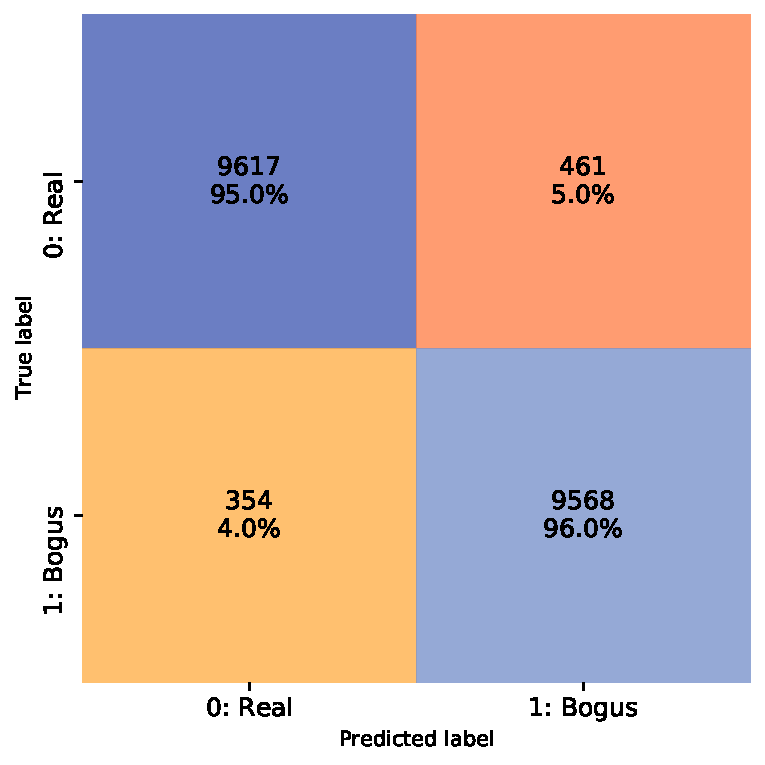
\includegraphics[width=0.5\linewidth]{figures/confusionmatrix_model_100K20KNERSC3CHANNELstam0-9CCCC_3s3DH.pdf}
    \caption{Confusion matrix (CM) for our testing data, a set composed of $10,078$ objects labeled as ``real'' and $9,922$ as ``bogus''.  Squares of the matrix, from the top left in the clockwise direction, indicate: True Positive (TP, \texttt{label = 0}, \texttt{prediction = 0} ), False Negative (FN, \texttt{label = 0}, \texttt{prediction = 1}), True Negatives (TN, \texttt{label = 1}, \texttt{prediction = 1}), and False Positive (FP, \texttt{label = 1}, \texttt{prediction = 0}). We note that here, somewhat unusually, 0 corresponds to ``real'' and ``positive'', and 1 to ``bogus'' and ``negative'', as we chose to remain consistent with the original labeling of the data presented in \citep{Goldstein_2015}. 
    The CM of our \textbf{\diabased } model with stacked third depth axis, \ie, (51, 51, 3) shows that from the $10,078$ transients labeled as ``real'', $9,617$ (\ie, 95\%) were correctly classified and the accuracy for the TN objects is even higher, at $96\%$.}\label{fig:vonfusiomatrix_3channel}
\end{figure*}